\chapter{Data acquisition and data structure}\label{dataacc}
This chapter is dedicated to the creation of a program that generates and visualizes the layout of Wi-Fi network topologies based on generated data and mined data.
The data will be used in chapter \ref{chap:clustering}, where some suggested distributed clustering algorithms are created and considered. Storing the data,
the data structure type, and finally how it can be visualized in a web application are also matters which will be addressed here. 

\section{Motivation}
There is an undoubtful need for data when developing a distributed clustering algorithm to facilitate group creation.
Surely a testbed could also do the trick, but it would require a large amount of routers. Maybe 100-200 for a low scale test, in a small geographical area,
preferably installed in residential apartment buildings. Not only would the creation of such a testbed require a vast amount of equipment, but there are 
some unsolved logical challenges as well. Like the communication protocol between routers, and maybe distributed consensus or some way to perform synchronization to communicate group memberships.
These problems are addressed in chapter \ref{chap:proto}.

Even if such challenges could be overcome, going directly from a concept idea to a large testbed in a master thesis  - without having any empirical indication of which approaches have merit, may not be a good use of time. Hence, the data is gathered with the motivation of being able to perform realistic calculations and do algorithm developement on a money-, and time budget. Lastly, the motivation behind mining real data, instead of generating everything, is to enhance the quality and believeability of the results produced. 

\section{Requirements and assumptions}
This section will cover the requirements and assumptions for a data generation-, and visualization program. 

\subsubsection{Background}
As presented in the background chapter: SSID, channel frequency, radio power, physical data rate and supported 802.11 standards are just a few of the properties
that makes up a wireless access point. Before deciding how to represent an access point in a network topology dataset, it is useful to
consider the state an access point would be in when group creation is performed.  

An access point is not in the transmission (CSMA/CA) state when performing channel allocation. This is simply due to the toughness of performing channel sensing without
having a channel to sense. So, which sate is it in then? Well, it is hard to say without having a bird's eye view of the protocol and algorithm architecture. A fully developed protocol
for distributed group-creation in residential deployed Wi-Fi is at the time of writing (and to the author's knowledge) non-existient.  Nor will a full-fledged architecture be presented in
this thesis (even though suggestions will be made at the end), so a couple of assumptions has to be made. 

\subsubsection{Assumptions}
The access points are in a state we can call the \textit{group discovery state}, where the goal is to find or create a group to be a part of. This state would occur before channel
allocation, as a major motivation for doing group creation in the first place is to be able to cleverly and collaboratively allocate channels within the group. 

Hence, to simulate group creation and discovery, many of the access point properties does not have to be considered. Actually it is only necessary to store two things:
\begin{itemize}
	\item Each access point's SSID, as a convenient way to provide a unique identification handle \footnote{In the real world this is of course not the case,
but we will enforce it in the computations. Actually it could just as well be called an unique id.}
	\item The list of neighboring access points that can be seen through a Wi-Fi interface scan on each access point, along with the observed signal strength of these APs.
\end{itemize}
Channel frequency, radio power and data rate are properties that impacts data transmission between clients and access points, and does not need to a 
part of this model. 

In all succeeding simulations it is assumed that all nodes are transmitting with equal strength, and that the environment is flat and obstacle free. 

\subsubsection{Requirements}
Unfortunately there is at the time of writing no publicly available data source that contains radio scans of a large amount of access points located in the same area.
This subsection describes the requirements for the simulation program that will both generate and represent Wi-Fi network topologies. Having a clear specificiation of program requirements
simplifies the programming stage and reduces the risk of feature creep. 

As a basis for the simulation, access points, hereupon also referred to as nodes, should be placed on a two-dimensional grid. Each dataset has to contain a set of nodes which has two coordinates $x$ and $y$, giving them a position on the grid. When all desired nodes are placed on a grid, the grid represents a network topology. It will then be possible to compute an
estimation of which nodes can hear each other over the Wi-Fi radio. In other words, a virtual network interface scan. All observed \textit{neighbour nodes} will be added to each node's
neighbour list. This neighbour list contains the names of all the nodes it can hear, and the signal strength levels measured in $-dBi$.

Additionally the following parameters should be variable in the topology generation program, depending on each test scenario:

\begin{itemize}
	\item Topology size with the possibility to give variable width of x- and y-axis as input arguments. These unit of the axes is meters. 
	\item Number of nodes to place on the topology
	\item Minimum distance between nodes (in meters). This is only to avoid unlikely placement and extreme interference of nodes that are placed on top of each other. 
	\item Minimum loudness measured in $-dBi$ for a node to account another node as a neighbour (e.g -100 is too low for anyone to hear).
\end{itemize}


	\section{Program design}\label{prog_design}
	The resulting program consists of two main functionalitites.

	The first functionality is creating a topology and generate nodes which are uniformly
	and randomly positioned on the network topology. The topology size, node count and minimum distance
	between nodes, are properties taken as input arguments to the program.

	The second functionality is performing the calculation of which nodes can actually observe each other over the radio.
	
	All neighbouring nodes observed by a node is added to its list of neighbours. The neighbour list contains the signal strength in $-dBi$ and the SSID of each neighbour.
	The interference levels between access points are calculated by iterating through every access point. For each node $N$ its x and y position is recorded,
	and then a second iteration through the nodes is initiated, resulting in a complexity of $O(N^2)$. For each node $n$ in the second iteration the distance $d$ in
	meters between $N$ and $n$ using Euclidean distance is calculated. The formula for isotropic antennas is described by Friis \cite{Friis46}, and can be used to
	derive the formula for free space path loss \cite{FSPL} that is as follows:
\[
	FSPL(dB) = 10\log_{10} \left( \frac{ (4 \pi f d)}{c} ^2 \right) 
\]	
	Where $d = distance$, $f = frequency$ and $c=constant$. The constant $c$ is used to account for different units. Meters is used to denominate distance in the program,
	and megahertz for the frequency. The resulting formula which will be implemented in the program is then: 
\[
	FSPL(dB) = 20\log_{10}\left( f \right)  + 20\log_{10} \left(d\right) - 27.55
\]	
	Pseudocode for the interference calculation can be seen in figure \ref{fig:dbiCreation}. 

	The resulting program, written in Python 3 \cite{Python3}, contains an importable \textit{topology class}. This way, for further testing we can use different data
	sources to get the positions of nodes, and only let the topology class compute the list of neighbours and standarize the data structure of a topology.

	The entire program can be viewed on GitHub: \newline
{\small \url{https://github.com/hansjny/GroupSimulations/blob/master/GenerateTopology.py}}

	

	\begin{figure}
		\begin{python}
#In topology class
def measureInterference(self):
 for nodeSubject in self._nodes:  
  for nodeObject in self._nodes:
    nodeSubject.calculateInterferenceTo(nodeObject) 

#In node class
def calculateInterferenceTo(self, nodeObject):
 if self == nodeObject:
  return
 dist = round(self.distanceTo(nodeObject))

#If  nodes have same coordinate, set high interference. 
 if (dist == 0):
  dBi = -40
 else:
  dBi  = self.measureDbi(dist) * -1

def measureDbi(self, dist):
 return (20 * math.log(self._frequency, 10)) + 
(20 * math.log(dist, 10)) - 27.55

\end{python}
\caption{Computing the interference between nodes}
\label{fig:dbiCreation}
\end{figure}

\section{Data output and visual representation} \label{simulationrep}
The result of the topology generation is stored in a JSON\cite{JSON} data file.
The data file contains the height and width of the the generated topology, as well
as the number of nodes.
A \verb|nodes| object consists of as many JSON node-objects as there are nodes. Figure \ref{fig:nodeStruct} illustrates the node structure and is an example of how a node with two neighbours will look.
			\begin{figure}
			\begin{minipage}{\linewidth}
			\begin{lstlisting}[language=json]
{
  "mapWidth": 100,
  "mapHeight": 100,
  "nodeCount": 3,
  "nodes": {
    1: {
    "posX": 50,
    "posY": 50, 
    "ssid": "NODE1", 
    "neighbourCount": 2, 
    "neighbours": {
      0: {
        "ssid": NODE2,
        "dbi": -77.23
        },
      1: {
        "ssid": NODE3,
        "dbi": -79.52
        }
      }
    }
  },
...
}
\end{lstlisting}
\end{minipage}
\caption{JSON output structure}
\label{fig:nodeStruct}

\end{figure}
The program can be run in the following way
\begin{verbatim}./GenerateTopology.py -n 500 -w 100 -h 100 --space 10 --dbi 85 \end{verbatim}
Which instructs the program to create a topology with 500 nodes. The topology should be 100 by 100 meters large, and there should be at least 10 meters
between each node. The $dbi$ parameter makes sure that only nodes which can be heard with a $-dBi$-value of $-85$ or larger should appear in the neighbour list. 
The output from this specific run is a 23.2 MB large file containing the resulting topology-data in JSON.

By writing a simple HTML and JavaScript browser application, the JSON can easily be parsed and visually represent the nodes on a grid.
The result after creating a topology and visualizing in the web applications can be seen in figure \ref{fig:randtop}

\begin{figure}[h]
\center
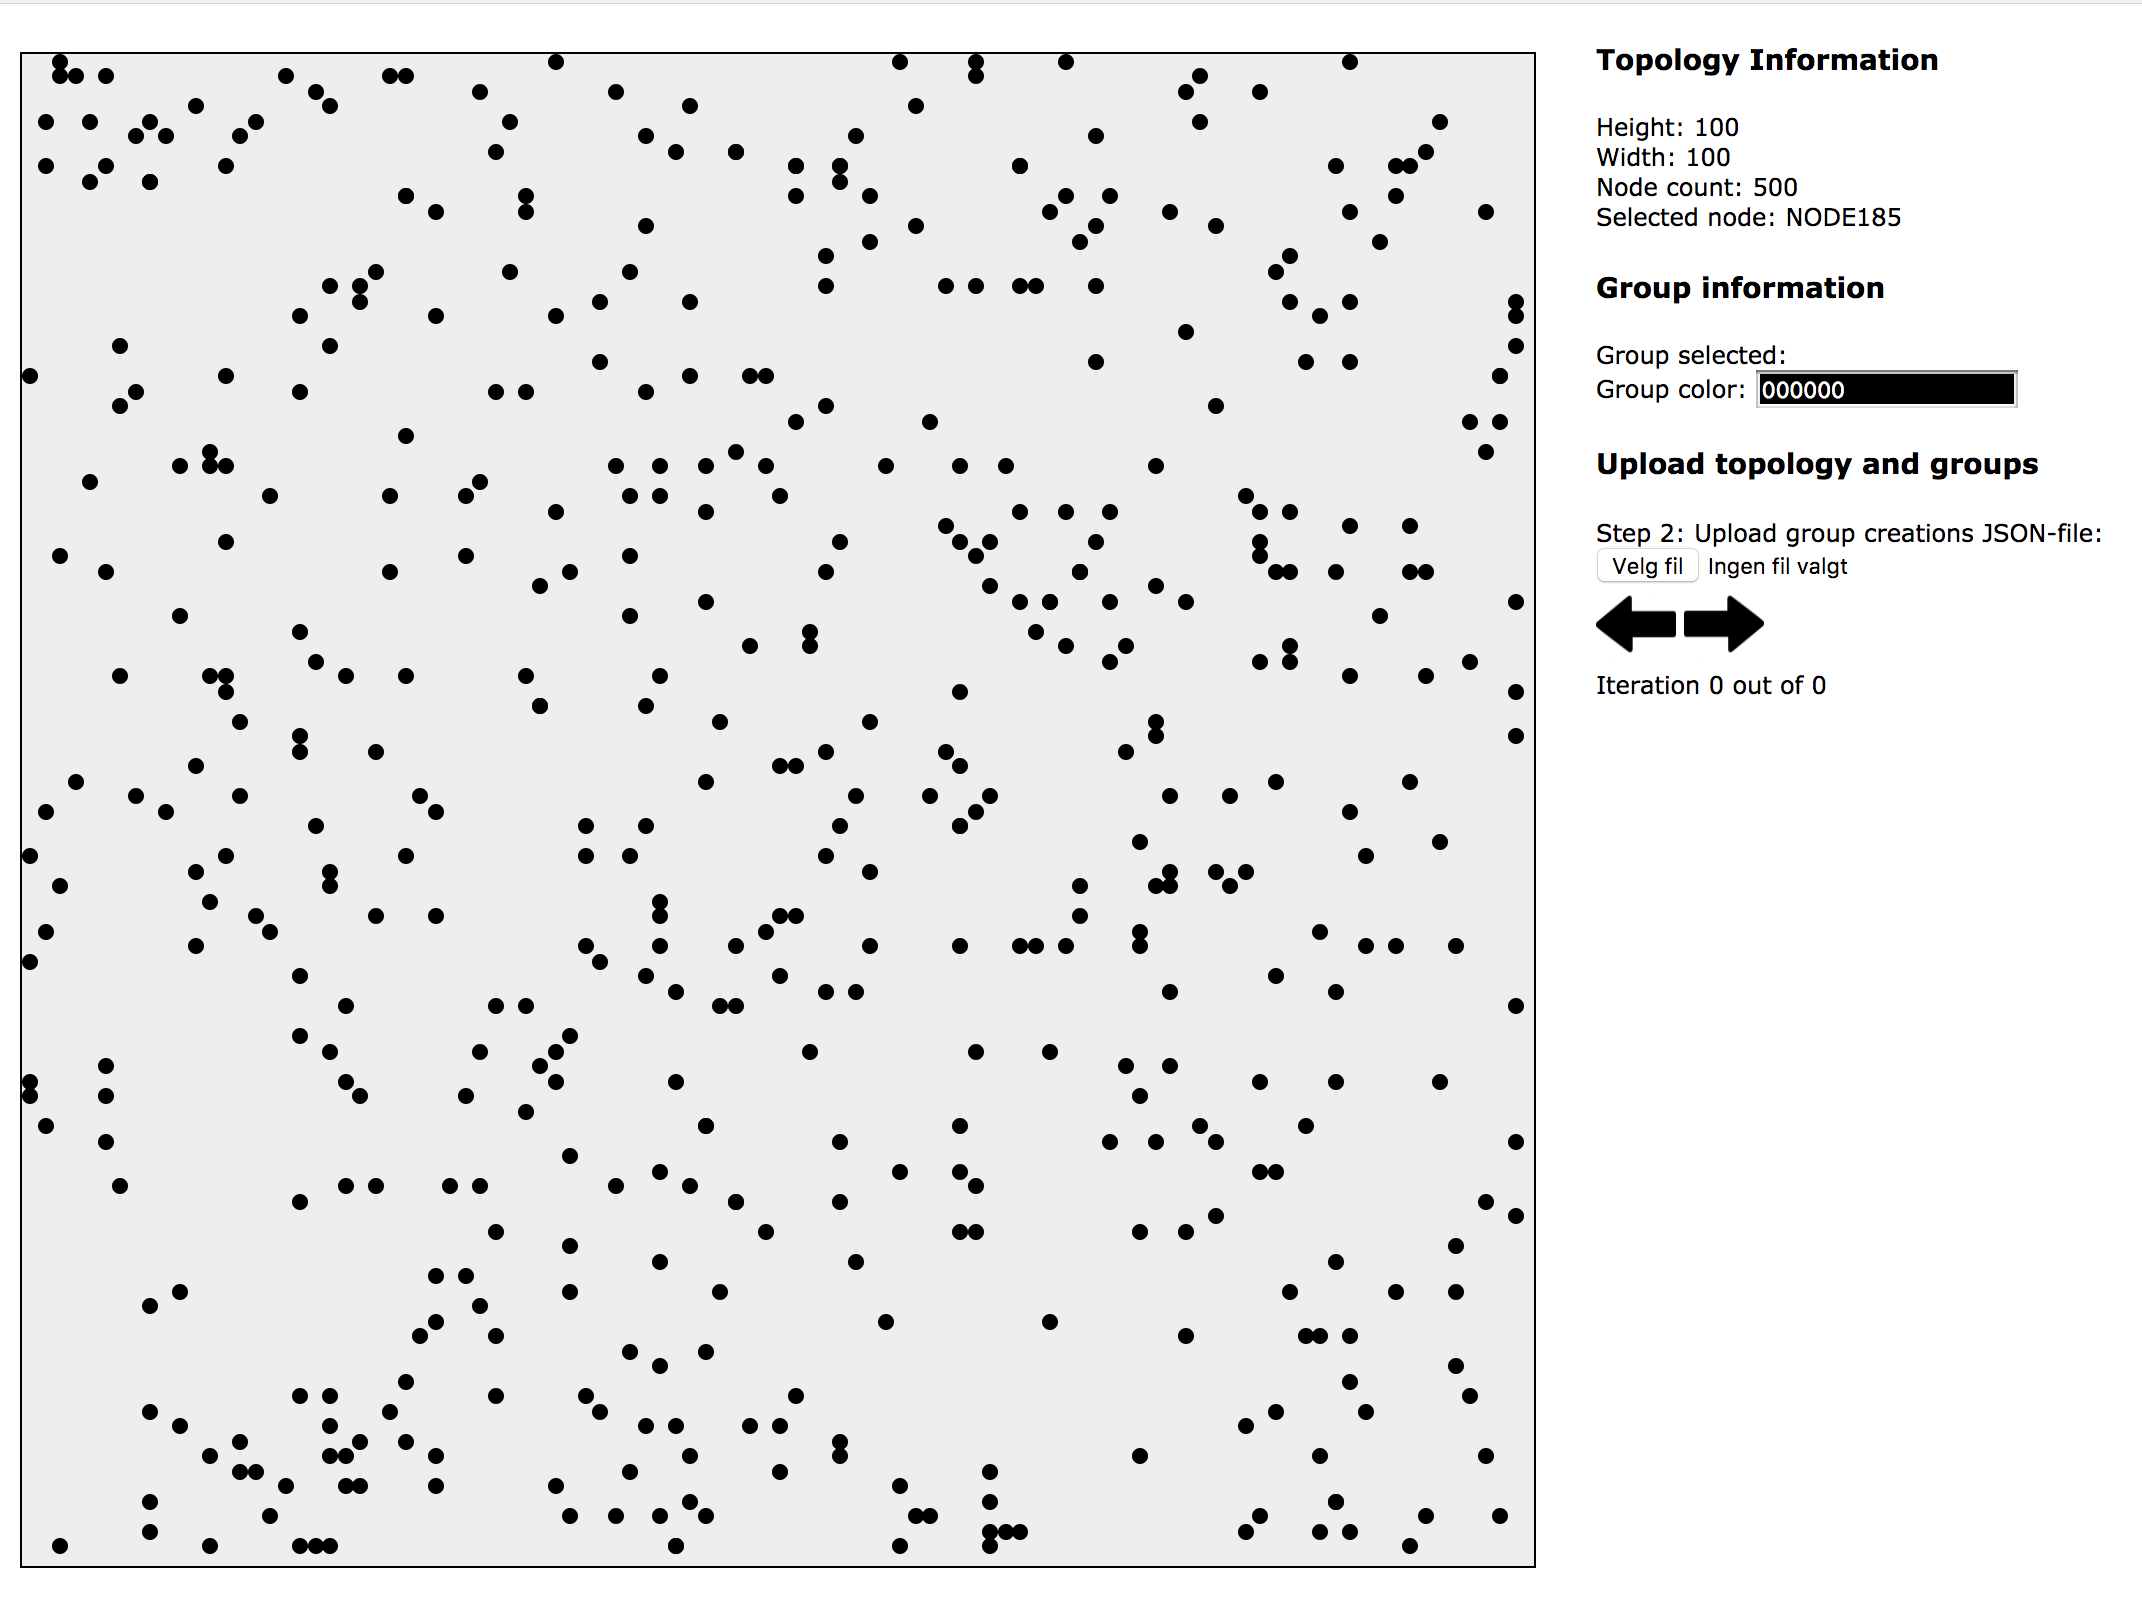
\includegraphics[scale=0.35]{Images/interface.png}
\caption{Generated topology with random, uniform distribution and the interface for viewing topologies}
\label{fig:randtop}
\end{figure}

\section{WiGLE}
WiGLE (Wireless Geographical Logging Engine) \cite{wigle} is a project started in 2001 which purpose is to gather information about wireless networks. All the information
they collect is user submitted stored in their database. Anyone can download an Android app developed and published by WiGLE, and use the app for wardriving\footnote{Wardriving is the act of tracking wireless networks using a laptop or a phone,	and then store the information about each network.},
	then submit the data to WiGLE's centralized database. The APs discovered can be viewed on an interactive map provided on WiGLE's website as seen in figure \ref{fig:wigfig} 
	All the data can also be accessed through a public API. Using their service is entirely free, but the
	amount of data that can be requested is throttled on a day-to-day basis. In the FAQ section on the website its written that the project openly supports research projects, 
	so after contacting them they upgraded the account to a higher daily data quota. This is needed for the data requests to fetch the topologies of interest. 

\begin{figure}[h]
	\center
	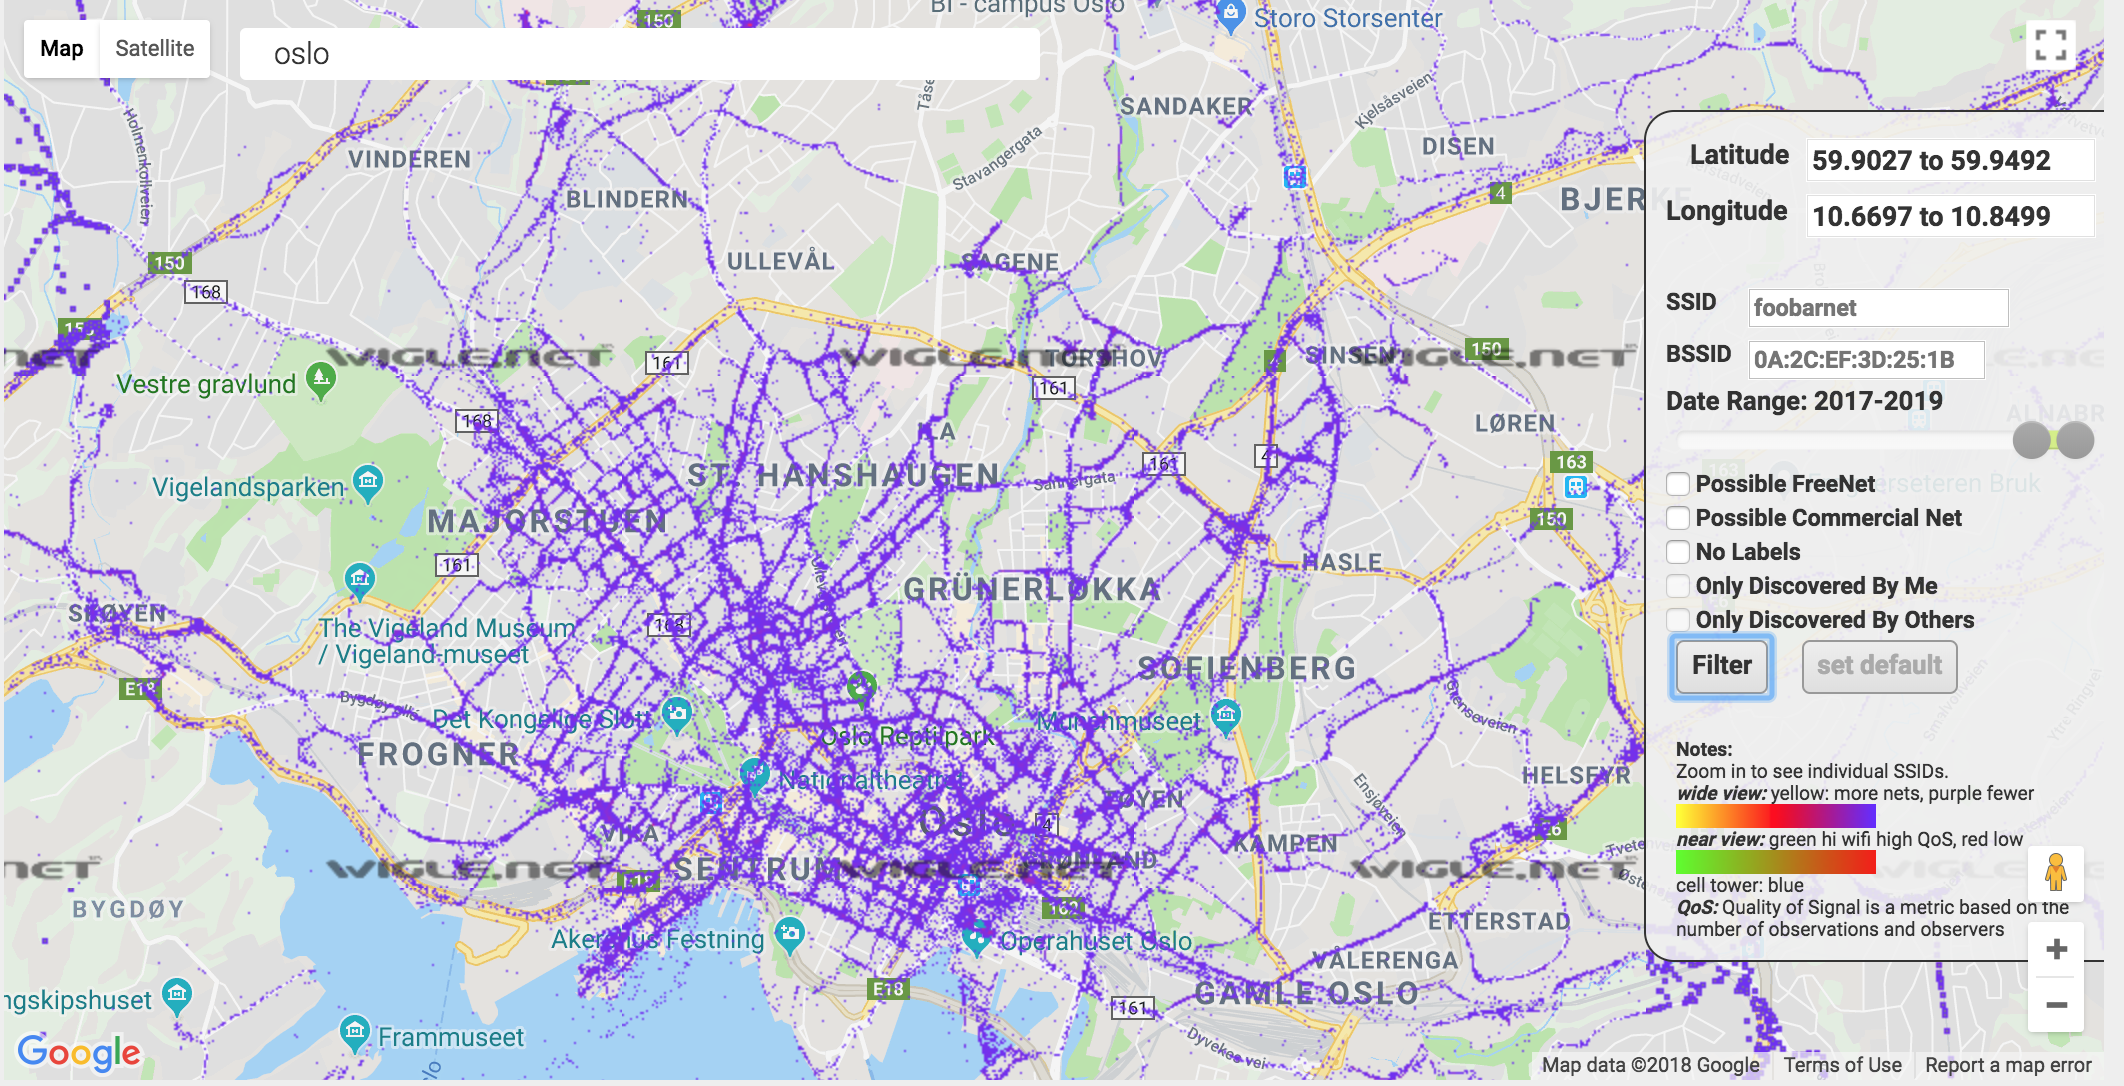
\includegraphics[scale=0.35]{Images/wigle.png}
	\caption{WiGLE map of Wi-Fi networks observed in Oslo from 2017-2018}
	\label{fig:wigfig}
\end{figure}


	As the physical location of each access point is estimated by WiGLE using weighted-centroid trilateration \cite{Sharma}, the location data is not necessarily always accurate:
	if the measurements of an access point signal strength is done in multiple places (in a way that a line between the measurement locations surrounds the access point),
	the access point location becomes very precise. On the other hand, if the measurements are taken on only one side of the access point,
	the measurements are heavily shifted towards that side. This tendency can be observed
	when zooming in on many Norwegian towns where most access points seem to be positioned on the road. This is obviously not right, but as most observations
	are most likely are done from the road when wardriving, this happens frequently. Figure \ref{fig:wiglediff} illustrates the big difference multiple observation points can make.

\begin{figure}
	\centering
		\subfloat[Few observation points in Ski, Norway]{{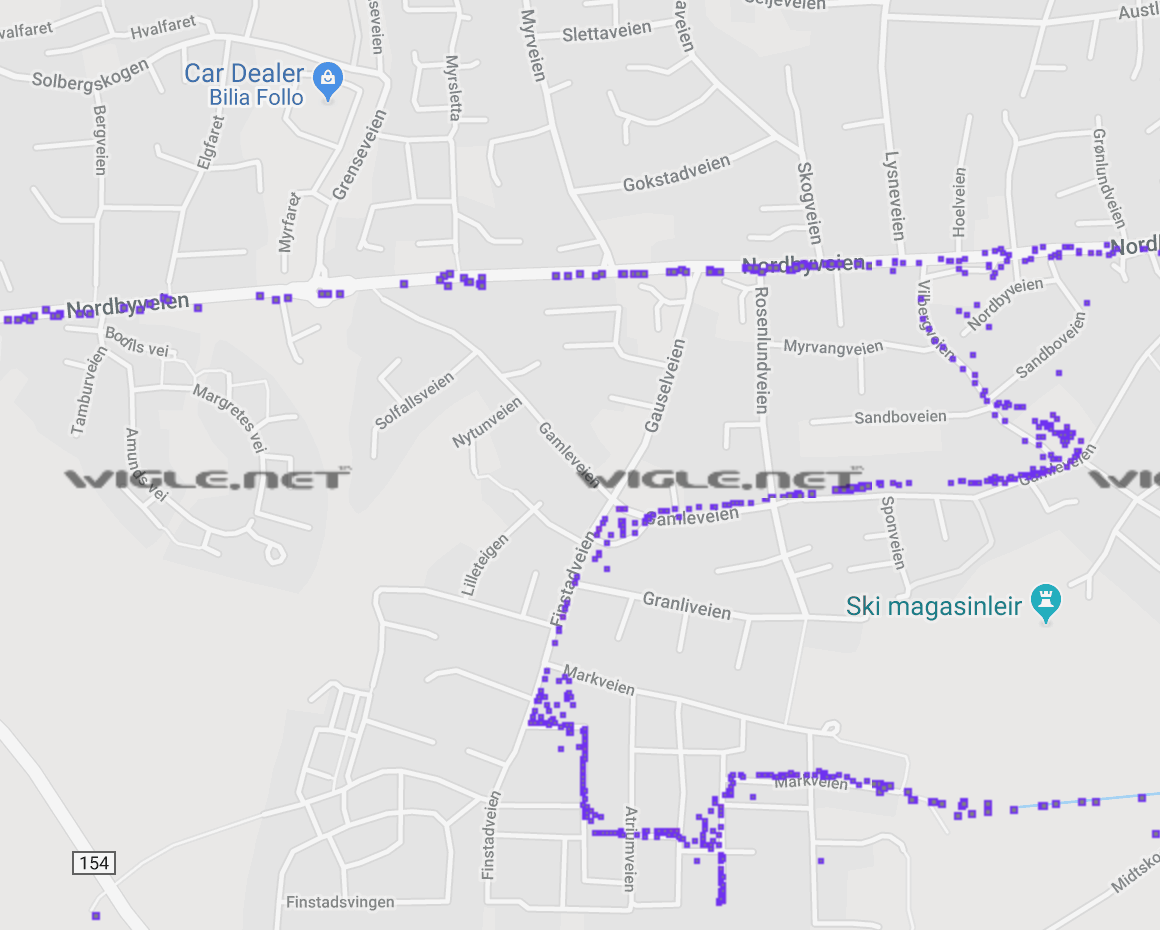
\includegraphics[width=6cm]{Images/wigleSki.png} }}%
		\qquad
		\subfloat[Several observations points in Manhattan, New York]{{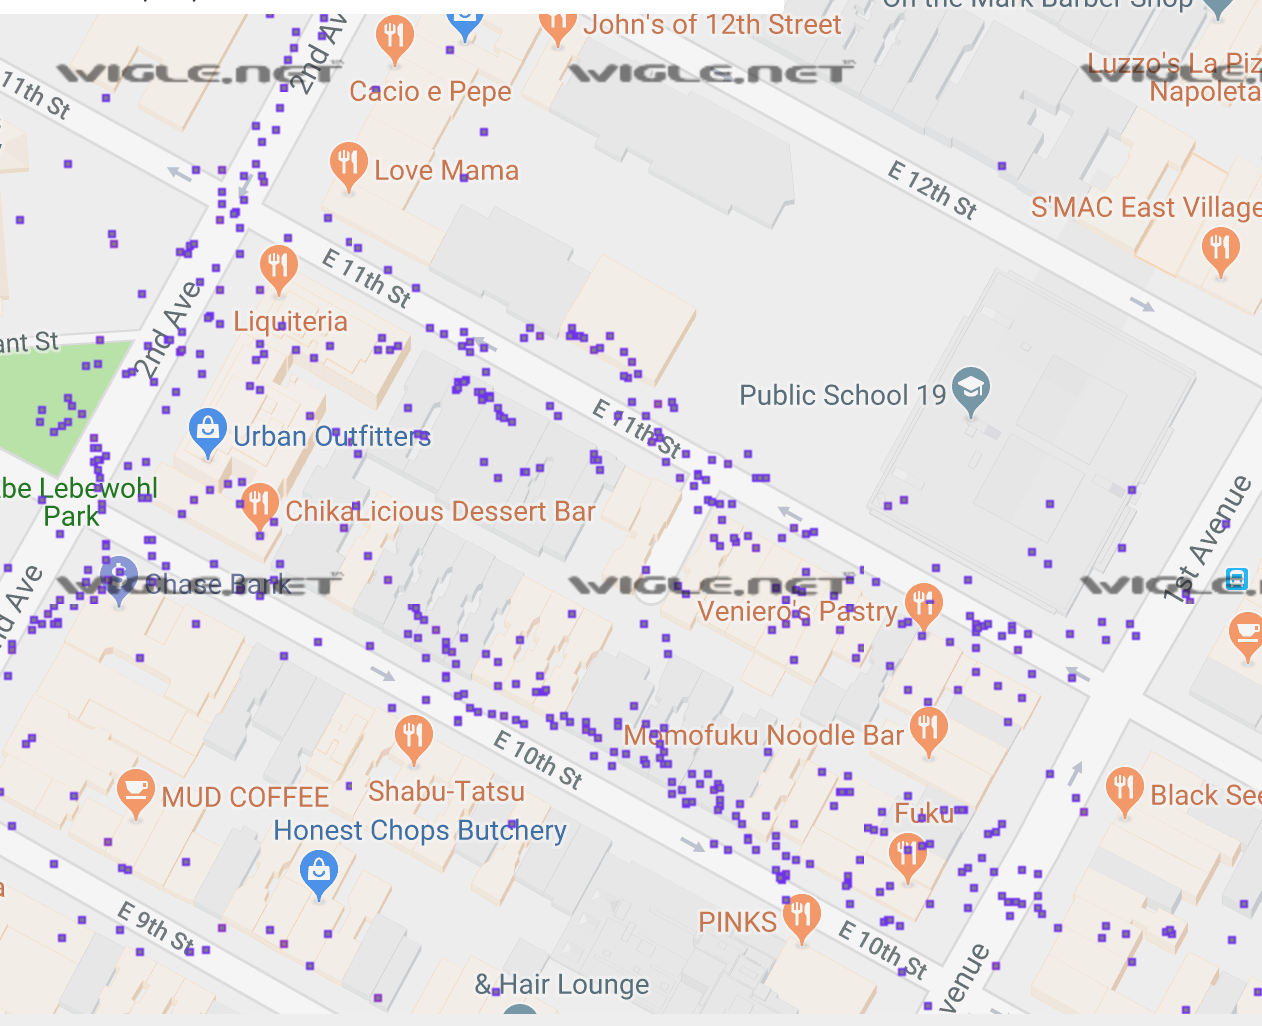
\includegraphics[width=6cm]{Images/wigleNy.png} }}%
		\caption{WiGLE accuracy}%
		\label{fig:wiglediff}%
\end{figure}

	Even though the data is not perfect, it is suited to impersonate the layout of real-life network topologies and give us a better understanding of how what access point
	clustering would look like in real-life. 

	\subsection{REST API}
	WiGLE has a REST API that can be used to retrieve information from their database. The API responds to requests with JSON data. It gives access to a
	number of services such as user profile management, large-scale statistical information about the collected data
	and more specific network searches. An interactive guide to the public API is available at \cite{WigleAPI}. 

	To retrieve data for the topology generation progam, the only required part of the API is the network search service. There are several ways an access point can be retrieved using
	the network search. For instance specific SSIDs can be queried, a range of coordinates, APs with a minimum signal level, or only query networks that are free to use. As 
	we are only rebuilding the network topology to fit the previously tailored data structure, all access points will be considered, and no filter parameter filters applied, except for coordinates.
	By issuing an API a request for nodes between two latitudes and two longitudes, the response is an array with AP objects within that area.  
	An API request will look something like what can be seen in figure \ref{fig:wigReq}.
	\begin{figure}
	\scriptsize
	\begin{lstlisting}[breaklines]
	 https://api.wigle.net/api/v2/network/search?first=0&latrange1=37.80846&latrange2=37.7467&longrange1=-122.5392&longrange2=-122.3813&start=0
	\end{lstlisting}
	\caption{Example of a Wigle API request}
	\label{fig:wigReq}
	\end{figure}

	The parameters $latrange1$ and $longrange1$ are the coordinates that marks the beginning of the area we are interested in and $latrange2$ and $longrange2$ marks the end. 
	To be meaningfully create a network topology based on the API request, information about \textit{all} access points within this range is desired. Alas, as it happens
	WiGLE returns at most 100 results per query. This means if there are more than 100 access points, the $start$
	parameter has to be changed. This parameter tells WiGLE at which offset we want to begin fetching data from. For instance a start value of $0$ means we fetch the first 100 access points, with indexes 0-99. A value of $100$ means that the next 100 APs in the range $100-199$ is fetched, and so on. The JSON response for a succesful request for one AP can be seen in figure \ref{fig:wigle}. 

	\begin{figure}[h]

	\begin{lstlisting}[language=json]
{
\subsection{Graph history}
	"userfound": false,
	"qos": 0,
	"comment": null,
	"lastupdt": "2015-12-22T17:49:34.000Z",
	"bcninterval": 0,
	"dhcp": "?",
	"lasttime": "2015-12-22T17:49:15.000Z",
	"trilong": 10.82792618,
	"netid": "5C:9E:FF:2B:54:84",
	"freenet": "?",
	"trilat": 62.2816925,
	"name": null,
	"firsttime": "2015-12-22T20:55:01.000Z",
	"type": "infra",
	"ssid": "NETGEAR23",
	"paynet": "?",
	"wep": "2",
	"transid": "20151222-00207",
	"channel": 52
}

\end{lstlisting}
\caption{REST API response with AP data}
\label{fig:wigle}
\end{figure}

The JSON-object in the response contains quite a lot of information about all of the APs retrieved. Most of this data is redundant information, but it is worth noting that some of it could be used to perfect the search. For instance the last updated parameter could
be a way to refine the access points retrieval, so that access points that has been long gone is not taken into consideration. The most valueable properties for us is $trilong$ and $trilat$. As the names suggest these contain the position calculated :wby the weighted-centroid triliteration. 

\subsection{The Haversine Formula}
As seen in the previous section, WiGLE provides data about the location of access points and a way for us to retrieve this data in a usable format. 
At this point we could create a program that operates directly on the longitudes and latitudes retrieved.
This program would also need to be able to use the FPSL formula on coordinates to compute the radio scans of each AP,
and to properly visualize the data we would have to reinstall the nodes on a globe. This implementation requires a lot of extra labour, and seems especially
redundant when we already have a working program that already has the aforementioned functionality.
The problem is that our previous work relies on a two dimensional Cartesian coordinate system.
To be able to reuse what we have have already built with, the geographic coordinates has to be translated into coordinates in Euclidean space to improve the accuracy.

The haversine formula \cite{virtues} is used to accurately compute the great-circle distance between two global coordinates.

\[
	d =2R sin^{-1} \left(\sqrt{ \left(sin\left(\frac{\varphi_2-\varphi_1}{2} \right)\right)^2 + cos(\varphi_1) * cos(\varphi_2) * sin\left(\left( \frac{\lambda_2 - \lambda_1}{2} \right)\right)^2} \right)
	%a = sin²(Δφ/2) + cos φ1 ⋅ cos φ2 ⋅ sin²(Δλ/2)
	%FSPL(dB) = 20\log_{10}\left( f \right)  + 20\log_{10} \left(d\right) - 27.55
\]	

Where $d$ is the distance between two latitudes $\varphi_1$ and $\varphi_2$ and two longitudes $\lambda_1$ and $\lambda_2$. $R$ is the radius of the
sphere, which in this context is the earth's radius. 

This can also be expressed with a two-parameter inverse tangent function \cite{chamberlain_2017}, as long as neither of the
parameters are zero. 

\begin{flalign}
	\nonumber a &= \left(sin\left(\frac{\varphi_2-\varphi_1}{2} \right)\right)^2 + cos(\varphi_1) * cos(\varphi_2) * sin\left(\left( \frac{\lambda_2 - \lambda_1}{2} \right)\right)^2 \\
	\nonumber c &= 2*atan2(\sqrt{a}, \sqrt{(1-a)}) \\
	\nonumber d &= c * R
	%a = sin²(Δφ/2) + cos φ1 ⋅ cos φ2 ⋅ sin²(Δλ/2
	%FSPL(dB) = 20\log_{10}\left( f \right)  + 20\log_{10} \left(d\right) - 27.55
\end{flalign}


The python implementation of the formula can be seen in figure \ref{fig:haversine}. It is imortant to note that the degrees taken as input
has to been converted to radians before inserting it in the formula. 

	\begin{figure}[H]
		\tiny
		\begin{python}
def distanceBetweenCoordinates(lat1, lat2, long1, long2):
	deltaLon = math.radians(long2 - long1)
	deltaLat = math.radians(lat2 - lat1)
	a = (math.sin(deltaLat / 2))**2 + math.cos(math.radians(lat1)) * math.cos(math.radians(lat2)) * (math.sin(deltaLon/2))**2
	c = 2 * math.atan2(math.sqrt(a), math.sqrt(1 - a)) 
	R = 6371000
	d = round(c * R)
	return d
	\end{python}
			\caption{Implementation of haversine distance}
			\label{fig:haversine}
	\end{figure}


This can be used to get the distance in meters between the boundaries of our area of interest. When the data is retrieved from
WiGLE we can use the specified coordinates to compute the size of the cartesian coordinate system.
The distance between the first latitude $\varphi_{start}$ and the second latitude $\varphi_{stop}$
is calculated. This is done by using the same longitude  $\lambda_1 = \lambda_2$, and returns the size of the x-axis in meters.
The opposite has to be done to get the size of the y-axis, using $\lambda_{start}$ and $\lambda_{stop}$ and equal longitudes.
The same approach can be used to place each node on the coordinate system, where the first set of the coordinates is
$\varphi_{start}$ and $\lambda_{start}$, and the second set is the coordinates of the AP.
\subsection{Data output}
The resulting python program \ref{appendix:wigleprogram}takes an output filename and two latitudes and two longitudes as input. It queries WiGLE's API for all the APs between these coordinates.
As long as the number of APs in the coordinate range does not exceed the daily data limit, all the data will be stored in a topology datastructure imported 
from the topology generation program in section \ref{prog_design}. The APs will be placed correctly relative to each other, with real world distance between them,
based on the coordinates of each AP. 

{{wigle data figure, overlaid map}}

